\section{Questão de Pesquisa} 
\label{sec:questao}

Para definir a questão de pesquisa norteadora deste trabalho foi utilizada a abordagem \textit{Goal Question Metric} (GQM), que propõe a especificação hierárquica de objetivos, questões e métricas de maneira \textit{top-down}, vide Figura \ref{fig:GOAL_QUESTION_METRIC}. O propósito desta abordagem é tornar o planejamento e a mensura dos objetivos de uma pesquisa em questões e métricas que embasem suas respostas. Seguindo essa estrutura e a adaptando para o contexto desta pesquisa, definiram-se as seguintes características: propósito, foco, objeto de estudo e ponto de vista (vide Tabela \ref{tab:gqm}). 

\begin{figure}[h] 
    \centering
    \caption{Estrutura do Modelo GQM}
    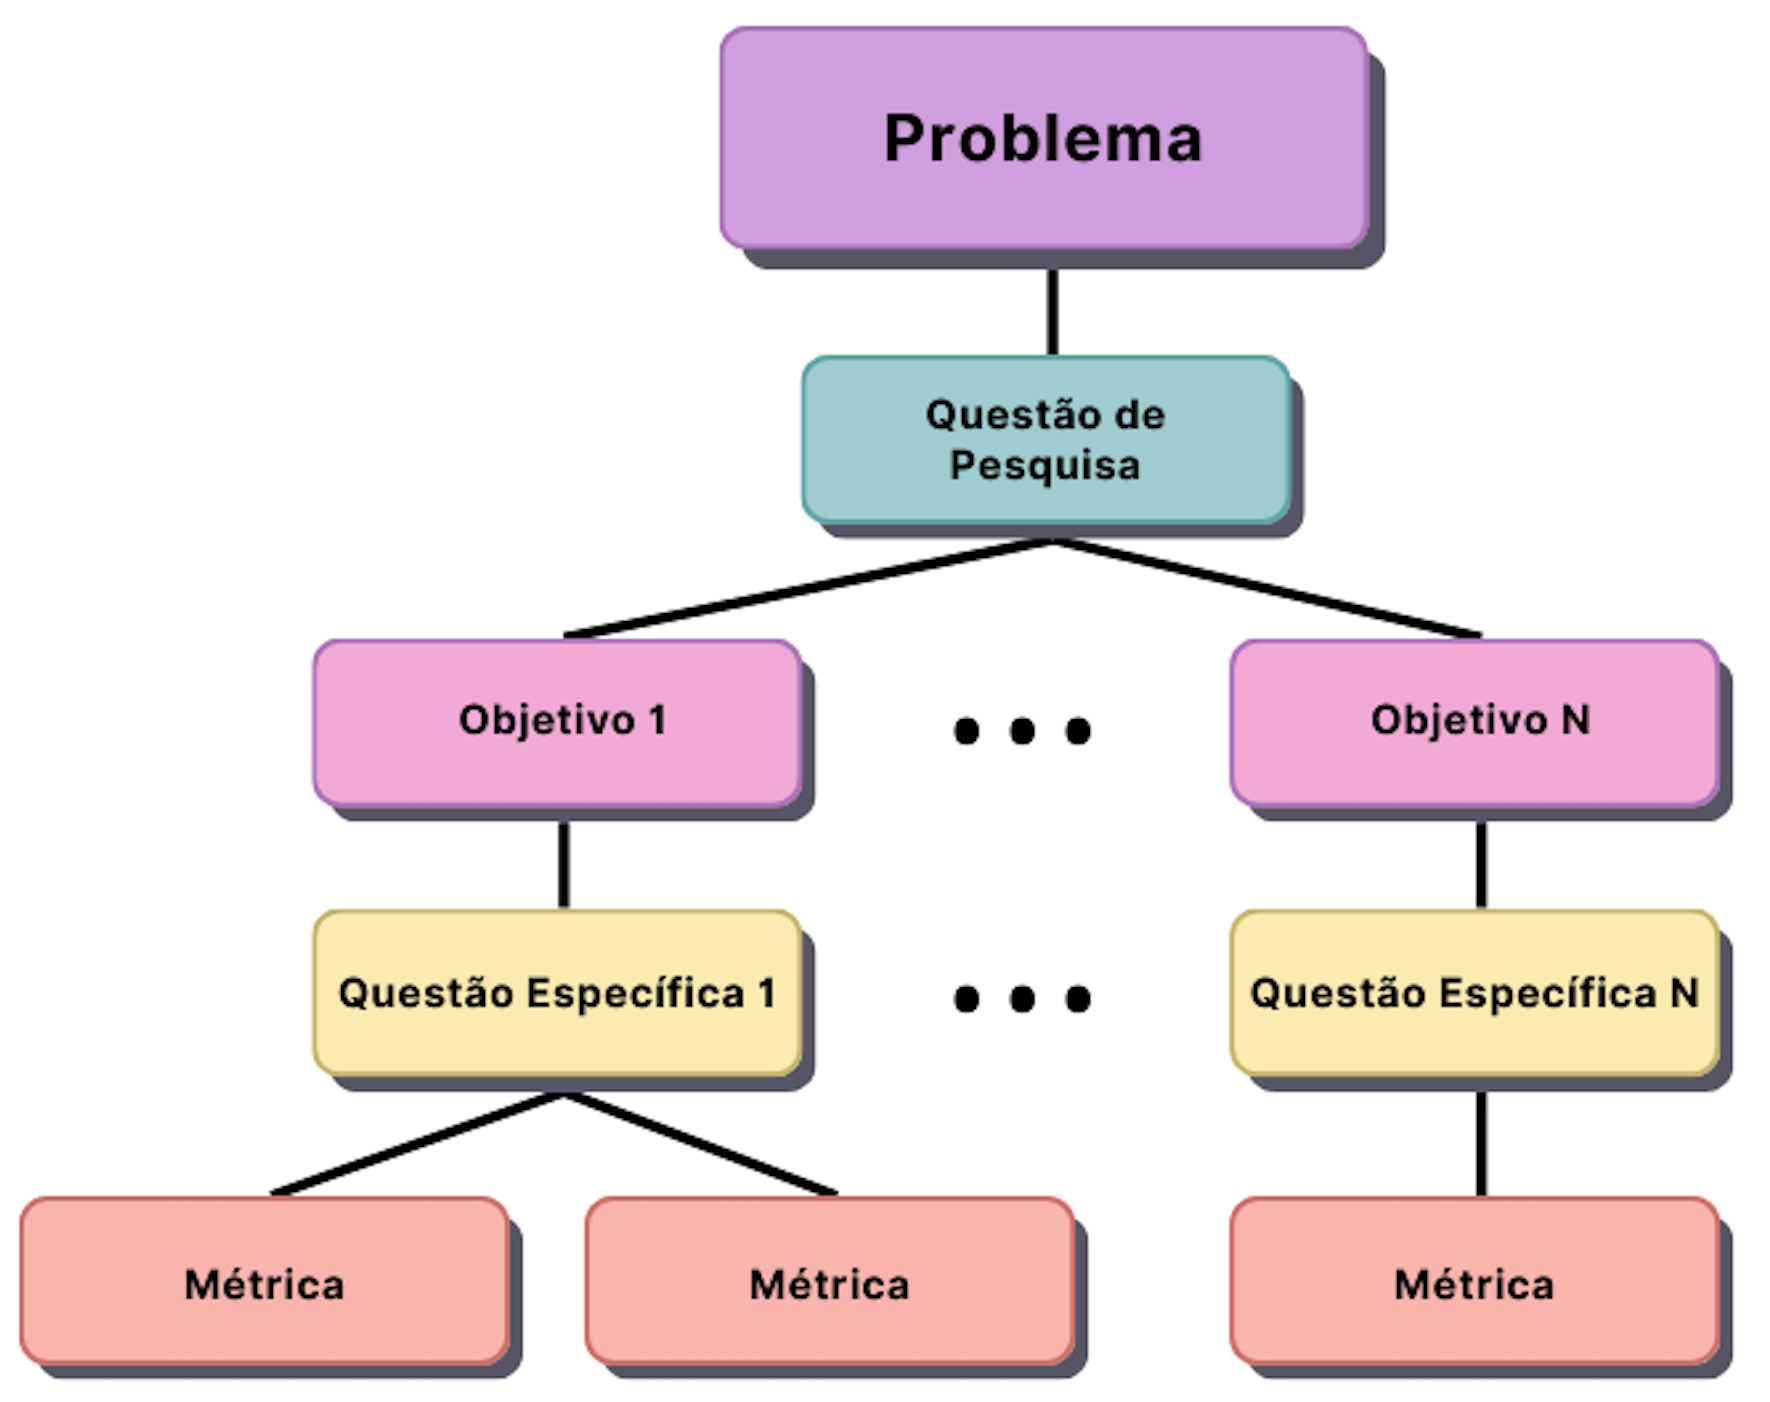
\includegraphics[width=0.75\textwidth]{figuras/gqm.png}

    \begin{center}
    \text Fonte: Adaptado de  \citeonline{basili_goal_1994}
    
    \end{center}
    \label{fig:GOAL_QUESTION_METRIC}
\end{figure}


\begin{table}[!h]
\centering
    \caption{Características de Definição da Questão de Pesquisa}
        \begin{tabular}{|p{4cm}|p{10cm}|}
            \hline
            \textbf{Característica} & \textbf{Valor} \\
            \hline
            Analisar & A adaptação de um processo de desenvolvimento \\
            Propósito & Avaliar \\
            Foco & Adoção de práticas de experimentação contínua para embasar a tomada de decisão na implantação de novas versões de um produto de \textit{software} \\
            Objeto de Estudo & Produto de Software \\
            Ponto de Vista & Pesquisador \\
            Contexto & Manutenção e evolução de um produto de \textit{software web}, em uma organização privada brasileira \\
            \hline
        \end{tabular}
    

    \begin{center}
        \text{Fonte: Adaptado de \citeonline{basili_goal_1994}}   
    \end{center}

    \label{tab:gqm}
\end{table}

Com isso, foi formulada a questão de pesquisa norteadora deste trabalho:

\begin{center}
    \textit{Como a adoção de práticas de experimentação contínua pode auxiliar a tomada de decisão sobre a implantação de novas versões de um produto de software web?}   
\end{center}
